\subsubsubsubsection{District starter}
\begin{figure}[h]
\centering
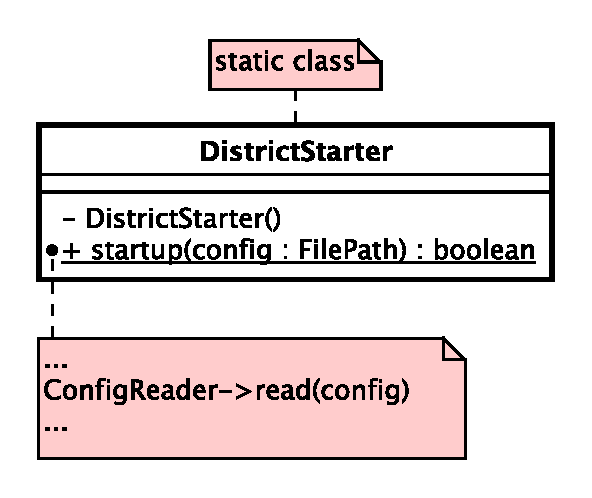
\includegraphics[scale=0.6,keepaspectratio]{images/solution/app/backend/district_starter.eps}
\caption{\pReactive::DistrictStarter}
\label{fig:sd-app-district-starter}
\end{figure}
\FloatBarrier
\begin{itemize}
  \item \textbf{\descr} \\
  It has the responsibility to boot the application layer.
  It is a static class because it is composed of only static methods.
  \item \textbf{\ops}
  \begin{itemize}
    \item \texttt{DistrictStarter()} \\
    Private and unique constructor because the class provides only static methods 
    so there are no reasons a client creates instances of it.
    \item[+] \texttt{\underline{startup(config: FilePath) : boolean}} \\
    Creates and boots all the entities of the district according to the 
    configuration file.
    Returns true if the process completes neatly, false otherwise.
    \item \texttt{\underline{load(config: FilePath) : boolean}} \\
    Creates all the entities of the district according to the 
    configuration file.
    Returns true if the process completes neatly, false otherwise.
    \item \texttt{\underline{loadStreets(streets: JSON) : boolean}} \\
    Creates all the streets of the district.
    Returns true if the process completes neatly, false otherwise.
    \item \texttt{\underline{loadCrossroads(crossroadsCollection: FilePath) : boolean}} \\
    Creates all the crossroads of the district. 
    Attaches each crossroads to the relative traffic light
    if specified so in the configuration file. 
    Returns true if the process completes neatly, false otherwise.
  \end{itemize}
\end{itemize} 
